\section{Generator-Optionen}
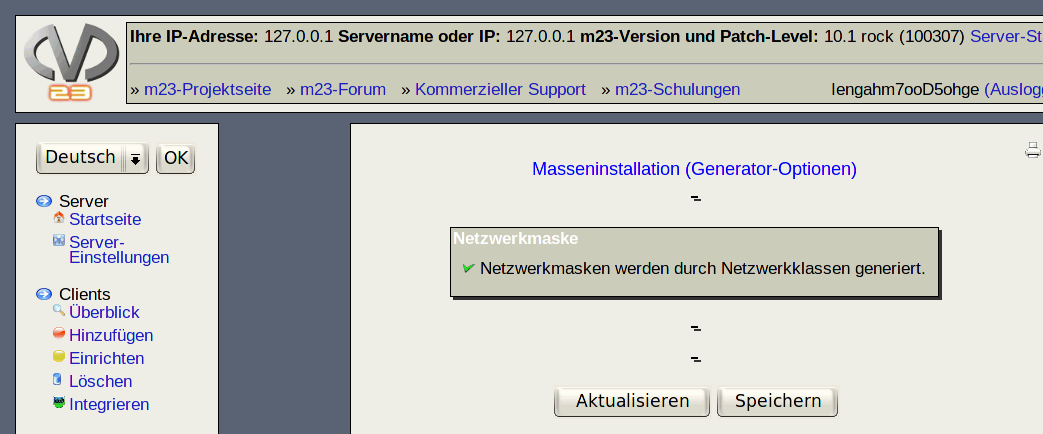
\includegraphics[scale=0.4]{/mdk/doc/manual/screenshots/de/mi_step3.png} \\
Hier k�nnen Sie die Parameter f�r die Generatoren der folgenden Eigenschaften festlegen:\\
\begin{itemize}
\item \textbf{Clientname}: Sie k�nnen hier den Client-Basis-Namen und eine Startnummer vorgeben. Die Clientnamen werden dann in der ben�tigten Anzahl nach dem Schema $\langle$Client-Basis-Name$\rangle$$\langle$fortlaufende Nummer$\rangle$ erstellt. Bereits vergebene Client-Namen werden bei der Generierung �bersprungen. Bsp.: Client-Basis-Name=m23client, Startnummer=12 generiert die Clientnamen m23client12, m23client13, ...\\
\item \textbf{Anmeldungsname}: Dies ist der Name, mit dem sich der Benutzer am Client anmelden kann. Es stehen zwei Methoden zur Generierung zur Verf�gung. Die inkrementelle Variante verh�lt sich identisch zur Erstellung bei \textit{"Clientname"}. Zus�tzlich ist das Bilden aus dem ersten Buchstaben des Vornamens und dem vollst�ndigen Nachnamen m�glich (\textit{"Aus Vor- und Nachnamen erstellen"}).\\
\item \textbf{Vorname}: Die Generierung der Vornamen (die zugleich die Loginnamen sind) geschieht analog zu den Clientnamen.\\
\item \textbf{IP-Adresse}: Legen sie hier die IP-Adressen-Bereiche fest, in denen nach freien IP-Adressen gesucht werden soll. Standardm��ig werden nur IP-Adressen generiert, die nicht bereits von m23-Clients benutzt werden. Sie k�nnen aber auch angeben, da� jede IP-Adresse vor der Verwendung "angepingt" werden soll. Sollte sich unter einer oder mehreren IP-Adressen ein Rechner melden, so werden diese IPs nicht verwendet.\\
\item \textbf{Netzwerkmaske}: Die Netzwerkmasken werden automatisch nach Schema der Netzwerk-Klassen berechnet. Dieses ist per Definition folgenderma�en:\\
\begin{tabular}{|c|c|c|}
\hline
Von & Bis & Netzwerkmaske\\
	 \hline
0.0.0.0 & 127.255.255.255 & 255.0.0.0\\
	 \hline
128.000.000.000 & 191.255.255.255 & 255.255.0.0\\
	 \hline
192.000.000.000 & 255.255.255.255 & 255.255.255.0\\
	 \hline
\end{tabular}
\item \textbf{Erstes Login}: F�r dieses Login k�nnen die Pa�w�rter komplett zuf�llig (\textit{"Zufalls-Pa�w�rter"}) oder nach einem zuf�lligen aber f�r Menschen leichter merkbaren Schema (\textit{"PwGen-Pa�w�rter"}) angelegt werden. Au�erdem kann die L�nge der generierten Pa�w�rter zwischen 6 und 8 Zeichen L�nge variiert werden. Es wird empfohlen, die voreingestellte L�nge von 8 beizubehalten.\\
\item \textbf{Benutzer-ID}: Legen Sie hier die Startnummer fest, ab der freie Benutzer-IDs gesucht und verwendet werden sollen.\\
\item \textbf{Gruppen-ID}: Legen Sie hier die Startnummer fest, ab der freie Gruppen-IDs gesucht und verwendet werden sollen.\\
\end{itemize}
